\documentclass[12pt]{report}

\usepackage[letterpaper, margin=1truein, footskip=.25in, twoside]{geometry}
\usepackage[utf8]{inputenc}
\usepackage[english]{babel}

\usepackage{setspace}
\doublespacing

% Header and footer
\usepackage{fancyhdr}
\pagestyle{fancy}
\fancyhead{}
\fancyhead[RO,LE]{\thepage}
\fancyhead[RE]{\it\leftmark}
\fancyhead[LO]{\it\rightmark}
\fancyfoot{}

% Figures and images
\usepackage{graphicx}
\graphicspath{ {images/} }
\usepackage{color}
\usepackage[font={small,it}]{caption}
\usepackage{epsfig}
\usepackage{epstopdf}

\usepackage{amsmath}
\usepackage{amsfonts}
\usepackage{amssymb}
\usepackage{url}
\usepackage{array}

\usepackage[inline]{enumitem}

\usepackage{amsthm}
\theoremstyle{plain}
\newtheorem{thm}{Theorem}[section]
\newtheorem{lem}[thm]{Lemma}
\newtheorem{prop}[thm]{Proposition}
\newtheorem{cor}{Corollary}[section]
\newtheorem{subclaim}{Claim}[subsubsection]

\theoremstyle{definition}
\newtheorem{defn}{Definition}[section]
\newtheorem{conj}{Conjecture}[section]
\newtheorem{exmp}{Example}[section]

\theoremstyle{remark}
\newtheorem*{rem}{Remark}
\newtheorem*{conv}{Convention}

\usepackage{tikz}
\usetikzlibrary{calc}

\usepackage{hyperref}

% Custom commands
\newcommand{\abs}[1]{\left|#1\right|}
\newcommand{\Conf}{\mathrm{Conf}}
\newcommand{\DConf}{\mathrm{Conf}^{\,\square}}
\newcommand{\UConf}{\mathrm{UConf}}
\newcommand{\DUConf}{\mathrm{UConf}^{\,\square}}
\newcommand{\Bd}{\mathrm{Bd}}
\newcommand{\closure}[1]{\overline{#1}}
\newcommand{\norm}[1]{\left\lVert#1\right\rVert}
\newcommand{\Lk}{\mathrm{Lk}}
\newcommand{\DLk}{\mathrm{Lk}_{\downarrow}}
\newcommand{\cone}{\mathrm{cone}}

\begin{document}

% --- Title, Abstract, and Acknowledgements ---
\begin{frame}
  \titlepage
\end{frame}
\clearpage\shipout\null
\pagenumbering{roman}
\chapter*{Abstract}
{\bf THESIS:} Graph Configuration Spaces and Braid Groups
\\{\bf STUDENT:} Zach Wilcher
\\{\bf DEGREE:} Master of Science
\\{\bf COLLEGE:} Sciences and Humanities
\\{\bf DATE:} May 2026
\\{\bf PAGES:} \pageref{LastPage}
\\
Given any space \(X\), the \(n\) point configuration space \(\Conf_n(X)\) is 
\(X^n - \Delta\), where \(\Delta\) is the diagonal in \(X^n\). 
Contrast this with the \(n\) point unordered configuration space \(\UConf_n(X) = \Conf_n(X) / S_n\)
where the quotient is obtained by permuting the coordinates of points in \(\Conf_n(X)\).
The fundamental groups of \(\Conf_n(X)\) and \(\UConf_n(X)\) are respectively known as the \(n\)-strand pure braid group
\(P_n(X)\) and the \(n\)-strand braid group \(B_n(X)\).
The base point will be omitted since the considered spaces are path connected.

\(B_n(\mathbb{R}^2)\) is also known as the Artin braid group and has applications
in motion planning, fluid mechanics, and quantum information theory.
Ghirst and Koditschek showed in 1999 that using a graph \(\Gamma\) as the underlying space has 
been applied to modeling the paths of automated guided vehicles.

Topologically, \(\Conf_n(\Gamma)\) is an interesting space in its own right. 
Abrams showed in 2000 that \(\Conf_2(\Gamma)\) is a surface if and only if \(\Gamma\)
is the complete \(5\) graph \(K_5\), or the bipartite graph \(K_{3,3}\).
By constructing the neighborhoods of each vertex in the configuration space
and computing the Euler characteristic, it can be shown
whether the space is a surface and what kind of surface it is.
The goals for this project are to 
find new examples of surfaces arising from \(\Conf_n(\Gamma)\) when \(n > 2\),
and to determine precisely which graphs yield surfaces when \(n > 2\).




\chapter*{Acknowledgements}
\tableofcontents
\clearpage\shipout\null
\pagenumbering{arabic}

% --- Content Chapters ---
\chapter{Configuration Spaces}
\section{Definitions and preliminary results}
% These definitions are presented in Abrams on page 10.
Given a topological space \(X\), the \(n\) point (topological) configuration space of \(X\) is
\(\Conf_n(X) = X^n - \Delta\) where \(\Delta\) is the diagonal in \(X^n\).

Treating a graph \(\Gamma\) as a topological space we can construct the
\(n\) point discretized or combinatorial configuration space \(\DConf_n(\Gamma)\) by 
% this diagonal needs elaboration.
removing a larger diagonal \(\Delta^{\square} = \{(e_1, \ldots, e_n) \mid x_i \cap x_j \neq \emptyset \text{ for some } i \neq j\}\)
from \(\Gamma^n\). Here \((e_1, \cdots, e_n)\) is any \(n\)-tuple of cells in \(\Gamma\).

Abrams showed in \cite{abrams2000configurationspaces} that \(\Conf_n(\Gamma)\) deformation retracts onto \(\DConf_n(\Gamma)\) and
that \(\DConf_n(\Gamma)\) is a cubical complex.
He also notes that any point in the
\(n\)-point configuration space is in one-to-one correspondence with a
collection of ``tokens'' placed on the graph. In this project, we will use a slightly different terminology and
and say ``particles'' instead of ``tokens.''

% TODO what is a cubical complex?
% make sure to define n-cubes and the gluing map

\begin{figure}[h!]
\centering
\begin{tikzpicture}
    \node (u1) at (2, 2) {\(u_1\)};
    \node (u2) at (4, 2) {\(u_2\)};
    \node (u3) at (3, 1) {\(u_3\)};
    \node (u4) at (3, 0) {\(u_4\)};
    \draw (u1) -- (u3);
    \draw (u2) -- (u3);
    \draw (u4) -- (u3);
\end{tikzpicture}
\caption{The \(Y\)-graph}
\label{fig:ygraph}
\end{figure}
Imagine \(2\) particles placed on the graph in \ref{fig:ygraph} at \(u_1\) and \(u_2\).  
In the topological configuration space, as the particle at \(u_1\) moves to \(u_3\)
the particle at \(u_2\) is free to simultaneously move to \(u_3\) as well. 
However, both particles would not be able to occupy the vertex \(u_3\) simultaneously.  
Compare this with the combinatorial configuration space, as the
particle at \(u_1\) moves to \(u_3\), the particle at \(u_2\) can not move at
all since the edges \(u_1 u_3\) and \(u_2 u_3\) intersect at \(u_3\) and points
with coordinates belonging to both edges are removed.

\begin{figure}[h!]
\centering
\begin{tikzpicture}
    \node (v1) at (0, 2) {\(v_1\)};
    \node (v2) at (0, 0) {\(v_2\)};
    \draw (v1) -- (v2);
    \node (u1) at (2, 2) {\(u_1\)};
    \node (u2) at (4, 2) {\(u_2\)};
    \node (u3) at (3, 1) {\(u_3\)};
    \node (u4) at (3, 0) {\(u_4\)};
    \draw (u1) -- (u3);
    \draw (u2) -- (u3);
    \draw (u4) -- (u3);
\end{tikzpicture}
\caption{An edge and a \(Y\)-graph}
\label{fig:edgeygraph}
\end{figure}
Now consider the graph in figure \ref{fig:edgeygraph} and put particles at \(v_1\) and \(u_3\).
As the particle at \(v_1\) moves to \(v_2\) there are three ways that the particle at \(u_3\) can move.
Since each way that the particle at \(u_3\) can move can be done simultaneously as the movement of the particle at \(v_1\),
the \(1\)-cell corresponding to the movement of the particle at \(v_1\) to \(v_2\)
borders three distinct \(2\)-cubes (see figure \ref{fig:threepagebook}).
We call this structure a \(3\)-page book.

\begin{figure}[h!]
\centering
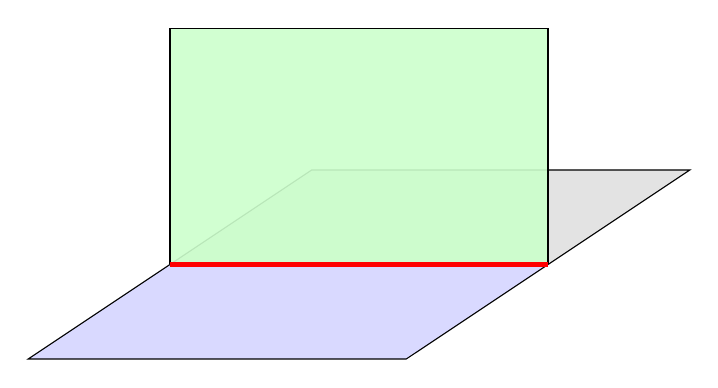
\begin{tikzpicture}[
    scale=1.2,
    % Define a 3D-like perspective by setting the coordinate vectors.
    % x goes to the right, y goes up, and z gives a sense of depth.
    z={(-0.6cm,-0.4cm)}, 
    x={(1cm,0cm)},      
    y={(0cm,1cm)}       
]
    % --- Define Coordinates for the vertices of the book ---
    
    % The spine is a 1-cell from O to A
    \coordinate (O) at (0,0,0);
    \coordinate (A) at (4,0,0);

    \coordinate (B_Back) at (4,0,-2.5);
    \coordinate (C_Back) at (0,0,-2.5);

    \coordinate (B_Front) at (4,0,2.5);
    \coordinate (C_Front) at (0,0,2.5);

    \coordinate (B_Up) at (4,2.5,0);
    \coordinate (C_Up) at (0,2.5,0);

    % Draw book pages
    \fill[gray!30, opacity=0.75] (O) -- (A) -- (B_Back) -- (C_Back) -- cycle;
    \draw (O) -- (C_Back) -- (B_Back) -- (A);

    \fill[blue!20, opacity=0.75] (O) -- (A) -- (B_Front) -- (C_Front) -- cycle;
    \draw (O) -- (C_Front) -- (B_Front) -- (A);

    \fill[green!20, opacity=0.9] (O) -- (A) -- (B_Up) -- (C_Up) -- cycle;
    \draw (O) -- (C_Up) -- (B_Up) -- (A);

    % --- Draw the Spine on top so it stands out ---
    \draw[line width=1.5pt, red] (O) -- (A);
\end{tikzpicture}
\caption{A 3-page book}
\label{fig:threepagebook}
\end{figure}

% It would make so much more sense if we excluded the covers of the book when counting the pages.
% Then, a book with more than 0 pages is not homeomorphic to a surface. 
% However, this would be an annoying substitution in later proofs.
\begin{defn}
    An \(n\)-page book is a collection of \(n\) \(2\)-cubes each glued along a common edge.
    This edge is called the spine of the book.
\end{defn}

Books are common structures found in configuration spaces.
One goal for this project is to determine which configuration spaces are surfaces.

\begin{thm}
A book with more than \(2\) pages is not a surface.
\end{thm}
\begin{proof}
Suppose there exists an \(n\)-page book that is a surface but \(n > 2\).
Let \(p\) be some point in the interior of the book's spine.
% pg. 225 Munkres states that an m-manifold X is a Hausdorff space such that for each point x in 
% X there exists a nehiborhood of x that is homeomorphic to an open subset of R^m.
% Let U be the neihborhood of p in X, V be the open subset of R^2, and \phi
% be the homeomorphism from U to V.
% Take some open disk B centered at \phi(p) in V such that \closure{B} \subseteq V
% restrict \phi to this open disk (this is okay to do in the codomain as \phi is a bijection).
Since the book is homeomorphic to a surface, there exists an open neighborhood \(U\) of \(p\)
which is homeomorphic to an open disk \(B\) in \(\mathbb{R}^2\).
Let \(\phi\) be a homeomorphism from \(\closure{U}\) to \(\closure{B}\) and \(S\) be the portion of book's spine inside of \(U\).
Notice that \(U \setminus S\) consists of \(n\) path components--one from each page of the book.
However,
\[
U\setminus S \cong \phi(U\setminus S) = B \setminus \phi(S).
\]

We claim that \(\phi(S)\) must separate \(B\) into two components.
To see this, first note that \(\phi(S)\) is a properly imbedded arc in \(B\) with \(\Bd(\phi(S))\) consisting of two
points on \(\Bd(B)\).
% homemorphisms map boundary points to boundary points, interior points to interior points, and exterior points to exterior points.
% This is common knowledge but a proof might be necessary TODO.
Since \(\Bd(B)\) is homeomorphic to a circle, there exists two different paths \(\alpha\) and \(\beta\) 
connecting these two points together (See Figure \ref{fig:thm:book_1_1}).

\begin{figure}[h!]
    \centering
    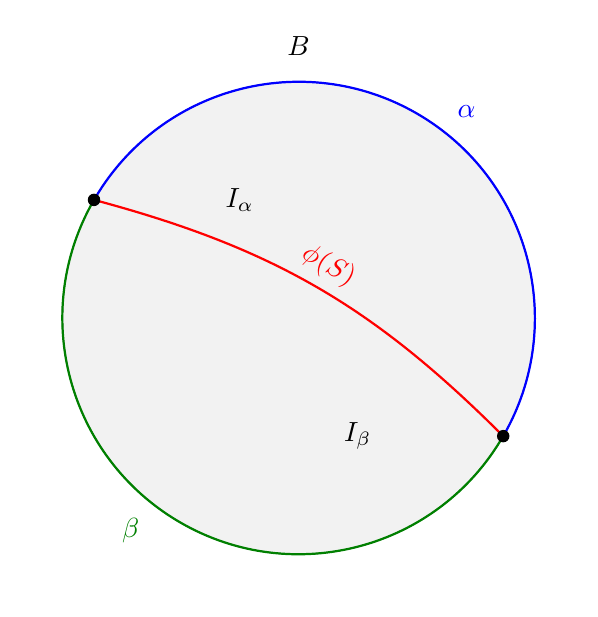
\begin{tikzpicture}[scale=1.5]
        % Define the main circle (the disk D^2) and fill it lightly
        \fill[gray!10] (0,0) circle (2cm);
        \draw (0,0) circle (2cm);
        \node at (0, 2.3) {\(B\)};

        % Define the start and end points of the arc on the boundary of the disk
        \coordinate (P1) at (150:2cm);
        \coordinate (P2) at (-30:2cm);

        % Draw the separating arc phi(S \cap U) with a distinct color
        \draw[thick, red] (P1) to[bend left=15] node[above, pos=0.5, sloped] {\(\phi(S)\)} (P2);

        % Draw the boundary path alpha
        \draw[thick, blue] (P2) arc (-30:150:2cm);
        \node[blue, above, xshift=18pt, yshift=-5pt] at (60:2cm) {\(\alpha\)};
        
        % Draw the boundary path beta
        \draw[thick, green!50!black] (P1) arc (150:330:2cm);
        \node[green!50!black, below, xshift=-18pt, yshift=5pt] at (240:2cm) {\(\beta\)};
        
        % Label the two regions separated by the arc
        \node at (-0.5, 1) {\(I_{\alpha}\)};
        \node at (0.5, -1) {\(I_{\beta}\)};
        
        % Mark the endpoints on the boundary
        \fill (P1) circle (1.5pt);
        \fill (P2) circle (1.5pt);

    \end{tikzpicture}
    \caption{The arc \(\phi(S)\) separates the open disk \(B\) into two components, \(I_{\alpha}\) and \(I_{\beta}\).}
    \label{fig:thm:book_1_1}
\end{figure}

The Jordan curve theorem guarantees that the simple closed curve \(\alpha \cup \phi(S)\) (resp. \(\beta \cup \phi(S)\))
separate \(B \setminus (\alpha \cup \phi(S))\) (resp. \(B \setminus (\beta \cup \phi(S))\)) into a bounded connected component
\(I_{\alpha}\) and an unbounded connected component \(O_{\alpha}\) (resp. \(I_{\beta}\) and \(O_{\beta}\)) when imbedded in \(\mathbb{R}^2\).
Notice \(B\setminus \phi(S) = I_{\alpha} \cup I_{\beta}\).
Since \(I_{\alpha} \subseteq O_{\beta}\) and \(I_{\beta} \cap O_{\beta} = \emptyset\),
we have that \(I_{\alpha} \cap I_{\beta} = \emptyset\).
So, \(I_{\alpha}\) and \(I_{\beta}\) form a separation of \(B\setminus \phi(S)\).
\end{proof}

Another common structure found found in graph configuration spaces are \(n\)-cubes.
Consider the graph in Figure \ref{fig:3edges} and imagine \(3\) particles placed at \(u_1\), \(v_1\), and \(w_1\).
Each particle can simultaneously move to \(u_2\), \(v_2\), and \(w_2\) resulting in \(3\)-cube in the configuration space (see Figure \ref{fig:3cube}).

\begin{figure}[h!]
    \centering
\begin{tikzpicture}
    \node (u1) at (0, 2) {\(u_1\)};
    \node (u2) at (0, 0) {\(u_2\)};
    \draw (u1) -- (u2);
    \node (v1) at (2, 2) {\(v_1\)};
    \node (v2) at (2, 0) {\(v_2\)};
    \draw (v1) -- (v2);
    \node (w1) at (4, 2) {\(w_1\)};
    \node (w2) at (4, 0) {\(w_2\)};
    \draw (w1) -- (w2);
\end{tikzpicture}
    \caption{Three edges}
    \label{fig:3edges}
\end{figure}

\begin{figure}[h!]
    \centering
    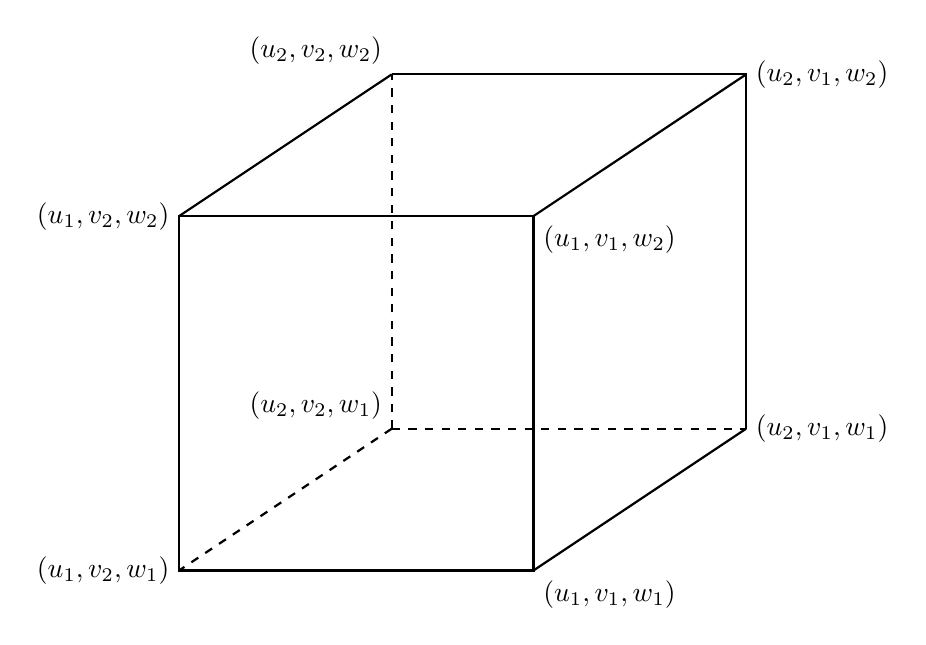
\begin{tikzpicture}[
    scale=1.5,
    % Define a 3D-like perspective by setting the coordinate vectors.
    % x goes to the right, y goes up, and z gives a sense of depth.
    x={(1cm,0cm)},
    y={(0cm,1cm)},
    z={(-0.6cm,-0.4cm)}
]
    % --- Style Definitions ---
    % Define styles for the cube's edges to make the code cleaner.
    % 'visible' edges are solid and thick.
    % 'hidden' edges are dashed and thick.
    \tikzstyle{visible} = [draw, thick, black]
    \tikzstyle{hidden} = [draw, thick, dashed, black]

    % --- Vertex Coordinates ---
    % Define the 8 vertices of the cube using (x,y,z) coordinates.
    % The side length of the cube is 3 units.
    \def\s{3}
    \coordinate (A) at (0,0,0);
    \coordinate (B) at (\s,0,0);
    \coordinate (C) at (\s,\s,0);
    \coordinate (D) at (0,\s,0);
    \coordinate (E) at (0,0,\s);
    \coordinate (F) at (\s,0,\s);
    \coordinate (G) at (\s,\s,\s);
    \coordinate (H) at (0,\s,\s);

    % --- Draw Hidden Edges ---
    % Draw the edges that would be obscured from view first. These are the
    % edges connected to the rearmost vertex (A).
    \draw[hidden] (A) -- (B);
    \draw[hidden] (A) -- (D);
    \draw[hidden] (A) -- (E);

    % --- Draw Visible Edges ---
    % Draw the visible edges on top of the hidden ones.
    \draw[visible] (B) -- (C) -- (D);
    \draw[visible] (E) -- (F) -- (G) -- (H) -- cycle;
    \draw[visible] (B) -- (F);
    \draw[visible] (C) -- (G);
    \draw[visible] (D) -- (H);

    % --- Optional: Label Vertices ---
    % Uncomment the following lines to add labels to each vertex.
    \node at (A) [above left] {\((u_2, v_2, w_1)\)};
    \node at (B) [right] {\((u_2, v_1, w_1)\)};
    \node at (C) [right] {\((u_2, v_1, w_2)\)};
    \node at (D) [above left] {\((u_2, v_2, w_2)\)};
    \node at (E) [left] {\((u_1, v_2, w_1)\)};
    \node at (F) [below right] {\((u_1, v_1, w_1)\)};
    \node at (G) [below right] {\((u_1, v_1, w_2)\)};
    \node at (H) [left] {\((u_1, v_2, w_2)\)};    
\end{tikzpicture}
\caption{3-cube}
\label{fig:3cube}
\end{figure}

Visually \(n\)-cubes are ``clearly'' not surfaces when \(n > 2\).
However, we can show this formally with an argument using the fundamental group.
\begin{thm}
\(n\)-cubes are not surfaces when \(n > 2\).
\end{thm}
\begin{proof}
    Suppose an \(n\)-cube \(C\) is a surface for some \(n > 2\).
    % imbed C in R^n
    Pick some point \(p\) in the interior of \(C\).
    Since \(C\) is a surface there exists some open ball \(B^n(p, \epsilon)\) in the interior of \(C\) such that 
    it is centered at \(p\) and is homeomorphic to some open neighborhood \(V\) of \(\mathbb{R}^2\).
    Let \(q\) be the point in \(V\) corresponding to \(p\).
    
    % TODO just use the fact that local simple connectedness fails after removing a point in D^2 but doesn't after removing a point in S^2.
\end{proof}

Books and cubes are the meat and potatos of the coming proofs.
\section{Computing the Euler characteristic of graph configuration spaces}
To compute the euler characteristic of an unorderd \(n\) point graph configuration space we need to count
for each \(0 \le k \le n\) the number of \(k\)-cubes present.
Without further mention \(E = E(\Gamma)\) and \(V = V(\Gamma)\).

A \(k\) cube exists if and only if \(k\) particles are free to move simultaneously while \(n - k\)
particles remain fixed.
Hence the general formula for the number of \(k\) cubes in \(\DUConf_n(\Gamma)\) is
\[
    \abs{\phi(k)} \cdot \begin{pmatrix}\abs{V} - 2k \\ n - k\end{pmatrix}
\]
where \(\phi(k)\) defined as follows.

\begin{defn}
\(\phi(k)\) is the collection consisting of all unordered sets of exactly \(k\) disjoint edges in \(\Gamma\)
where \(\phi(0) = \{\emptyset\}\).
\end{defn}

Note that we define \(\phi(0) = \{\emptyset\}\) so that \(\abs{\phi(0)} = 1\).
With this definition, \(\abs{\phi(k)}\) is also known as the number of ``\(k\)-matchings'' in \(\Gamma\).

Counting the number of \(k\)-matchings for small graphs can be done efficiently 
with a simple sweep over all \(k\) combinations of edges.
However, for general larger graphs this computation quickly becomes unwieldly.

% TODO read/cite Mark Jerrum's paper "Two-dimensional monomer-dimer systems are computationally intractable"
% where he proves computing the matching polynomial for planar graphs is P# ?
% TODO: reference program actually used to make computations? It's trivial especially now with AI hah

\begin{figure}[h!]
\centering
\begin{tabular}{c | c | c}
   \(\Gamma\) & \(n\) & \(\chi(\DUConf_n(\Gamma))\) \\
   \hline
   \(K_5\) & 2 & -5 \\
   \(K_{3,3}\) & 2 & -3 \\
   \(K_5\) & 3 & -5 \\
   \(\Theta_4\) & 3 & -4 \\
   \(K_{3,3}\) & 4 & -3
\end{tabular}
\label{fig:euler_characteristics}
\caption{Euler characteristic of certain unordered graph configuration spaces.}
\end{figure}

A workaround for this computational challenge is determing the Euler characteristic of certain classes of graphs.
In \cite{appiah2024algebraicstructurehyperbolicgraph} the ``pulsar'' graph was defined.


\begin{figure}[h!]
    \centering
\begin{tikzpicture}[scale=1]
    % Define the two main suspension vertices, positioned closer together
    \node (a1) at (0, 1) {\(a_1\)};
    \node (a2) at (0, -1) {\(a_2\)};

    % Define the intermediate vertices for the 'm' paths
    \node (b1) at (-1, 0) {\(b_1\)};
    \node (bm) at (1, 0) {\(b_m\)};
    \node at (0,0) {\(\dots\)};

    % Draw the edges for the 'm' paths, passing through the b_i nodes
    \draw (a1) to[out=180, in=90] (b1);
    \draw (b1) to[out=270, in=180] (a2);

    \draw (a1) to[out=0, in=90] (bm);
    \draw (bm) to[out=270, in=0] (a2);

    % Define vertices for the 'n1' rays attached to a1, spread out as in the drawing
    \node (c1) at (-1, 2) {\(c_1\)};
    \node (c1p) at (-2, 3) {\(c'_1\)};
    \node (cn1) at (1, 2) {\(c_{n_1}\)};
    \node (cn1p) at (2, 3) {\(c'_{n_1}\)};
    \node at (0, 2.5) {\(\dots\)};

    % Draw edges for the 'n1' rays
    \draw (a1) -- (c1);
    \draw (c1) -- (c1p);
    \draw (a1) -- (cn1);
    \draw (cn1) -- (cn1p);

    % Define vertices for the 'n2' rays attached to a2, also spread out
    \node (d1) at (-1, -2) {\(d_1\)};
    \node (d1p) at (-2, -3) {\(d'_1\)};
    \node (dn2) at (1, -2) {\(d_{n_2}\)};
    \node (dn2p) at (2, -3) {\(d'_{n_2}\)};
    \node at (0, -2.5) {\(\dots\)};

    % Draw edges for the 'n2' rays
    \draw (a2) -- (d1);
    \draw (d1) -- (d1p);
    \draw (a2) -- (dn2);
    \draw (dn2) -- (dn2p);
\end{tikzpicture}
\label{fig:pulsargraph}
\caption{The Pulsar graph \(\mathcal{P}_{m,n_1,n_2}\)}
\end{figure}

\begin{thm}
    \label{thm:pulsargrapheuler}
    The Euler characteristic of \(\DUConf_{3}(\mathcal{P}_{m,n_1,n_2})\) is
    \[
    \frac{m^{3}}{6} - \frac{3 m^{2}}{2} - \frac{m n_{1}^{2}}{2} - \frac{3 m n_{1}}{2} - \frac{m n_{2}^{2}}{2} - \frac{3 m n_{2}}{2} + \frac{7 m}{3} - \frac{n_{1}^{3}}{3} + \frac{7 n_{1}}{3} - \frac{n_{2}^{3}}{3} + \frac{7 n_{2}}{3}.
    \]
\end{thm}
\begin{proof}
%TODO: all we really have to do is explain the argument for the 2 and 3 matchings.
\end{proof}

\begin{rem}
Substituting in \(n_1 = 0\) and \(n_2 = 0\) the pular graph becomes \(\Theta_m\).
So, 
the euler characteristic of \(\DUConf_3(\Theta_m)\) is
\[
\frac{m^{3}}{6} - \frac{3 m^{2}}{2} + \frac{7 m}{3}
\]
This aligns with results in section 4 of \cite{appiah2024algebraicstructurehyperbolicgraph}.
\end{rem}
\chapter{Surfaces}
% Input sections
\section{Background}
In his thesis \cite{abrams2000configurationspaces}, Abrams asked:
For which \(n\) and \(\Gamma\) is \(\DConf_n(\Gamma)\) homeomorphic to a closed manifold?
He establishes a partial answer to this question in Corollary 5.8: 
if \(\Gamma\) is a connected graph
without loops and \(\DConf_n(\Gamma)\) is homeomorphic to a closed
\(n\)-dimensional manifold, then either \(n = 1\) and \(\Gamma\) is a cycle, or
\(n = 2\) and \(\Gamma\) is \(K_5\) or \(K_{3,3}\).

Advised by Peter Haskell, Praphat Fernandes in his undergraduate thesis
demonstrates that if \(\Gamma\) is a simple graph and \(\DConf_2(\Gamma)\)
is a \(2\)-psuedomanifold without boundary the following are true.
\begin{enumerate}
    \item If \(\Gamma\) contains a valence 4 vertex, then \(\Gamma\) is \(K_5\).
    \item If every vertex in \(\Gamma\) has valence 3, then \(\Gamma\) is \(K_{3,3}\).
\end{enumerate}
This recovers Abrams' result about when \(\DConf_2(\Gamma)\) 
is a \(2\)-manifold, as Praphat also shows that
if \(\Gamma\) is simple and \(\DConf_2(\Gamma)\) is a 2-psuedomanifold without boundary,
then the valence of every vertex in \(\Gamma\) is between 3 and 4,
and \(\DConf_2(\Gamma)\) is a 2-manifold. Also advised by Peter Haskell, Molly Ison in \cite{ison2005two} 
extends Fernandes' work in her masters thesis to 2-psuedomanifolds with boundary.

% TODO: is it though?
The question for when \(\DConf_n(\Gamma)\) is an \(m\)-manifold 
when \(n \neq m\) remains open.

In Example 4.3 in \cite{ko2012characteristics}, it is shown that \(\DConf_3(\Theta_4)\)
is a closed orientable surface of genus 3 by computing its fundamental group and using the
fact that discretized configuration spaces are \(K(\pi, 1)\) spaces.
This result is recovered in \cite{appiah2024algebraicstructurehyperbolicgraph}
with a strictly combinatorial argument.

The goal of this chapter is to
answer for what \(\Gamma\) and what \(n\) is
\(\DConf_n(\Gamma)\) is a \(2\)-manifold without boundary.
\section{Ruling out other graphs}
The example graphs in the previous section are in fact the only connected graphs
whose discretized configuration spaces are surfaces.

\begin{lem}
\label{lem:is_surface_0}
If \(\DConf_n(\Gamma)\) is an \(m\)-manifold with or without boundary, then \(\Gamma\) has at least \(n+m\) vertices and \(n \ge m\).
\end{lem}
\begin{proof}
    If \(\Gamma\) has less than \(n\) vertices, then \(\DConf_n(\Gamma)\) is empty;
    so, suppose \(\Gamma\) has at least \(n\) vertices.
    If \(\Gamma\) has less than \(n + m\) vertices, then
    for any configuration of \(n\) particles on \(\Gamma\)
    at most \(m-1\) particles can simultaneously move.
    Since exactly \(m\) particles need to be able to simultaneously move for an \(m\)-cube 
    to exist in \(\DConf_n(\Gamma)\), no configuration in \(\DConf_n(\Gamma)\)
    can have a neighborhood homeomorphic to an open set in \(\mathbb{R}^m\).

    Similarly, if \(n < m\), then there are not enough particles that can simultaneously move
    for an \(m\)-cube to exist in \(\DConf_n(\Gamma)\). So, \(n \ge m\). 
\end{proof}

\begin{lem}
    \label{lem:is_connected_0}
    If \(\DConf_n(\Gamma)\) is connected, then \(\Gamma\) has at least \(n + 1\) vertices
    and \(\Gamma\) is connected.
\end{lem}
\begin{proof}
    Suppose \(\DConf_n(\Gamma)\) is connected.
    If \(\Gamma\) has less than \(n + 1\) vertices, then \(\DConf_n(\Gamma)\) is either empty or
    consists of \(n!\) isolated points; so, \(\Gamma\) must have at least \(n+1\) vertices.

    Let \(v_1\) and \(v_2\) be distinct vertices in \(\Gamma\).
    To construct a path in \(\Gamma\) between \(v_1\) and \(v_2\), first let \(w_1, \ldots, w_{n-1}\)
    be \(n-1\) vertices in \(\Gamma\) distinct from \(v_1\) and \(v_2\).
    Next, since \(\DConf_n(\Gamma)\) is connected, there must be a path \(\gamma\)
    in \(\DConf_n(\Gamma)\) between the configurations
    \((v_1, w_1, \ldots, w_{n-1})\) and \((v_2, w_1, \ldots, w_{n-1})\).
    The path \(\gamma\) corresponds to a sequence of (potentially simultaneous) movements of particles on \(\Gamma\).
    In particular the particle at \(v_1\) must be able to eventually move to \(v_2\).
    The sequence of edges traveled by this particle gives a path in \(\Gamma\) between \(v_1\) and \(v_2\).
\end{proof}


\begin{lem}
    \label{lem:is_surface_1}
    Suppose \(\DConf_n(\Gamma)\) is a \(2\)-manifold without boundary and let
    \(v_1\) and \(w_1\) be adjacent vertices in \(\Gamma\). For any collection
    of \(n-1\) vertices \(\{v_2, \cdots, v_n\}\) in \(\Gamma - \{v_1, w_1\}\)
    there exists exactly two edges \(e_1 = v_i w_2\) and \(e_2 = v_j w_3\) such that
    \begin{enumerate}[label=(\roman*)]
        \item \(v_i\) and \(v_j\) belong to \(\{v_2, \cdots, v_n\}\)
        \item \(w_2\) and \(w_3\) fall outside of \(\{w_1, v_1, \cdots, v_n\}\)
        \item exactly one of the following hold in Figure \ref{fig:lem:is_surface_1_1}.
    \end{enumerate}

\begin{figure}[h!]
    \centering
        \begin{enumerate*}[label=(\arabic*)]
            \item \label{fig:lem:is_surface_1_1:1}
            \begin{minipage}{.3\textwidth}
                \centering
                \(v_i = v_j\) \textit{and} \(w_2 \neq w_3\) \\
                \vspace{1em}
                \begin{tikzpicture}
                \node (v1) at (0,2) {\(v_1\)};
                \node (w1) at (0,0) {\(w_1\)};
                \draw (v1) -- (w1);
                \node (vi) at (3, 2) {\(v_i\)};
                \node (w2) at (2, 0) {\(w_2\)};
                \node (w3) at (4, 0) {\(w_3\)};
                \draw (vi) -- (w2) node[midway, left] {\(e_1\)};
                \draw (vi) -- (w3) node[midway, right] {\(e_2\)};
                \end{tikzpicture} 
            \end{minipage}
            \hspace{3em}

            \item \label{fig:lem:is_surface_1_1:2}
            \begin{minipage}{.3\textwidth}
                \centering
                \(w_2 = w_3\) \textit{and} \(v_i \neq v_j\) \\
                \vspace{1em}
                \begin{tikzpicture}
                    \node (v1) at (0,2) {\(v_1\)};
                    \node (w1) at (0,0) {\(w_1\)};
                    \draw (v1) -- (w1);
                    \node (vi) at (2, 2) {\(v_i\)};
                    \node (vj) at (4, 2) {\(v_j\)};
                    \node (w2) at (3, 0) {\(w_2\)};

                    \draw (vi) -- (w2) node[midway, left] {\(e_1\)};
                    \draw (vj) -- (w2) node[midway, right] {\(e_2\)};
                \end{tikzpicture}
            \end{minipage}
        \end{enumerate*}
    \caption{Lemma \ref{lem:is_surface_1} possibilities.}
    \label{fig:lem:is_surface_1_1}
\end{figure}
\end{lem}
\begin{proof}
    Let \(v_2, \cdots, v_n\) be \(n-1\) vertices in \(\Gamma - \{v_1, w_1\}\).   
    Now, put a particle at each of the vertices \(v_1, \cdots, v_n\).
    Since no particle exists at \(w_1\) and \(v_1\) is adjacent to \(w_1\), 
    the particle at \(v_1\) can travel from \(v_1\) to \(w_1\).
    This particles movement corresponds to a \(1\)-cube in \(\DConf_n(\Gamma)\).
    Since the configuration space is a \(2\)-manifold without boundary, 
    this \(1\)-cube must border exactly two distinct \(2\)-cubes.
    For this \(1\)-cube to border some \(2\)-cube,
    there must be another particle at some vertex \(v_i \in \{v_2, \ldots, v_n\}\) that can move to some vertex
    \(w_2 \not \in \{w_1, v_1, \ldots, v_n\}\).
    Furthermore, since this \(1\)-cube needs to border two \(2\)-cubes, 
    the movement of the particle from \(v_i\) to \(w_2\) cannot be the only other movement in addition to
    the movement of the particle from \(v_1\) to \(w_1\). 
    Let \(v_j\) and \(w_3\) be the vertices corresponding to this other movement.
    
    Notice that if \(v_i \neq v_j\) and \(w_2 \neq w_3\), then as the particle at \(v_1\) travels to \(w_1\), the particles
    at \(v_i\) and \(v_j\) can simultaneously travel to \(w_2\) and \(w_3\) respectively. These three simultaneous movements correspond
    to a \(3\)-cube in \(\DConf_n(\Gamma)\) with the point \((v_1, \cdots, v_n)\) as a corner.
    Since \(\DConf_n(\Gamma)\) is assumed to be a \(2\)-manifold and \(e_1\) and \(e_2\) are distinct, 
    the result follows.
\end{proof}

The idea that every \(1\)-cube in our cubical complex must border exactly two distinct \(2\)-cubes
for it to be homeomorphic to a \(2\)-manifold without boundary can be generalized to
\(m\)-manifolds without boundary. In the next section we explore this idea further.
% TODO DELETE THIS IF WE DON'T ACTUALLY EXPLORE IT FURTHER!!!!!!!!!!!!!!
% Also, put a link to this section if we do.

\begin{lem}
    \label{lem:is_surface_2}
    Suppose \(\DConf_n(\Gamma)\) is a \(2\)-manifold without boundary for some \(n \ge 3\) and let \(v_1\) and \(w_1\) be adjacent vertices in \(\Gamma\).
    Let \(\{v_2, \cdots, v_n\}\) be a collection of \(n-1\) vertices in \(\Gamma - \{v_1, w_1\}\) 
    and \(e_1 = v_i w_2\), \(e_2 = v_j w_3\) be the edges guaranteed
    from applying Lemma \ref{lem:is_surface_1} to \(\{v_2, \cdots, v_n\}\) in \(\Gamma - \{v_1, w_1\}\).
    Then, exactly one of the following is true.
    \begin{enumerate}
        \item \(n = 3\) and these edges belong to a \(Y\)-graph in \(\Gamma - \{v_1, w_1\}\) with two vertices not in \(\{v_2, \cdots, v_n\}\).
        \item \(e_1\) and \(e_2\) belong to a \(3\)-cycle in \(\Gamma - \{v_1, w_1\}\) with exactly two vertices not in \(\{v_2, \cdots, v_n\}\).
        \item \(e_1\) and \(e_2\) belong to an \(r\)-cycle in \(\Gamma - \{v_1, w_1\}\) with exactly one vertex not in \(\{v_2, \cdots, v_n\}\) and \(3 \le r \le n\).
    \end{enumerate}
\end{lem}
\begin{proof}
    The argument proceeds by cases on the possibilities for the edges \(e_1\) and \(e_2\).
    
    \textbf{Case 1:} \(v_i = v_j\) (See \ref{fig:lem:is_surface_1_1:1} in Figure \ref{fig:lem:is_surface_1_1}). 
    In this case, \(e_1 = v_i w_2\) and \(e_2 = v_i w_3\). 
    Let \(v_k\) be some vertex in \(\{v_2, \cdots, v_n\}\setminus\{v_i\}\).
    Applying Lemma \ref{lem:is_surface_1} to \(\{w_2, v_2, \cdots, v_n\}\setminus\{v_k\}\) in \(\Gamma - \{v_1, w_1\}\),
    we obtain two new edges \(e_3\) and \(e_4\).
    Since \(e_2\) already connects \(v_i\) to \(w_3\) and there must be exactly two edges
    with exactly one endpoint in \(\{w_2, v_2, \cdots, v_n\}\setminus\{v_k\}\),
    one of \(e_3\) or \(e_4\) is \(e_2\). 
    Without a loss of generality suppose \(e_4 = e_2\).
    Since \(e_3\) must share an endpoint with \(e_4 = e_2\), it follows that \(e_3\) has either \(v_i\) as an endpoint or \(w_3\) as an endpoint (See Figure \ref{fig:lem:is_surface_2_0}).
    \begin{figure}[h!]
        \centering
        \begin{tikzpicture}
            \node (v1) at (0,2) {\(v_1\)};
            \node (w1) at (0,0) {\(w_1\)};
            \draw (v1) -- (w1);
            \node (vi) at (3, 2) {\(v_i\)};
            \node (w2) at (2, 0) {\(w_2\)};
            \node (w3) at (4, 0) {\(w_3\)};
            \draw (vi) -- (w2) node[midway, left] {\(e_1\)};
            \draw (vi) -- (w3) node[midway, right] {\(e_2\)};
            
            \node (vk) at (5, 2) {\(?\)};
            \draw (vi) -- (vk) node[midway, above] {\(e_3\)};
        \end{tikzpicture}
        \quad\quad
        \begin{tikzpicture}
            \node (v1) at (0,2) {\(v_1\)};
            \node (w1) at (0,0) {\(w_1\)};
            \draw (v1) -- (w1);
            \node (vi) at (3, 2) {\(v_i\)};
            \node (w2) at (2, 0) {\(w_2\)};
            \node (w3) at (4, 0) {\(w_3\)};
            \node (q) at (6, 0) {\(?\)};
            \draw (vi) -- (w2) node[midway, left] {\(e_1\)};
            \draw (vi) -- (w3) node[midway, right] {\(e_2\)};
            \draw (q) -- (w3) node[midway, below] {\(e_3\)};
            
        \end{tikzpicture}
        \caption{Possibilities if \(v_i = v_j\)}
        \label{fig:lem:is_surface_2_0}
    \end{figure}

    Lemma \ref{lem:is_surface_1} guarantees two facts about the edges we have so far.
    \begin{enumerate}
        \item \(e_1\) and \(e_2\) are the only edges with exactly one endpoint in \(\{v_2, \cdots, v_n\}\).
        \item \(e_3\) and \(e_4 = e_2\) are the only edges with exactly one endpoint in \(\{w_2, v_2, \cdots, v_n\}\setminus\{v_k\}\).
    \end{enumerate}
    We claim that if \(e_3\) has \(v_i\) as an endpoint, then \(v_k\) must be the other endpoint of \(e_3\)
    (see the graph on the left in Figure \ref{fig:lem:is_surface_2_1}).
    To verify this claim, suppose \(e_3\) has \(v_i\) as an endpoint and let \(v^*\) be the other endpoint of \(e_3\).
    Since \(e_3 \neq e_1\) and \(e_3 \neq e_2\) but \(e_3\) has \(v_i\) as an endpoint, the first fact above 
    guarantees that \(v^* \in \{v_2, \cdots, v_n\}\).
    The second fact guarantees that \(v^* \not \in \{w_2, v_2, \cdots, v_n\}\setminus\{v_k\}\).
    Hence,
    \[
        v^* \in \left(V(\Gamma - \{v_1, w_1\})\setminus(\{w_2, v_2, \cdots, v_n\}\setminus\{v_k\})\right) \cap \{v_2, \cdots, v_n\} = \{v_k\}.
    \]

    Moreover, if \(e_3\) has \(v_i\) as an endpoint, 
    then since \(v_k\) was arbitrary, 
    every vertex in \(\{v_2, \cdots, v_n\}\setminus\{v_i\}\) is adjacent to \(v_i\).

    So, if \(n > 3\) then there are two vertices say \(v_k\) and \(v_r\) in the set \(\{v_2, \cdots, v_n\}\) that are distinct but adjacent to \(v_i\).
    Put particles at each vertex in the set \(\{w_2, v_1, \cdots, v_n\}\setminus\{v_i\}\).
    As the particle at \(v_1\) moves to \(w_1\), any one particle in the set \(\{w_2, v_k, v_r\}\) can move to \(v_i\).
    These particles movements result in a book in the configuration space whose spine corresponds to the movement of the particle at \(v_1\) to \(w_1\).
    Therefore if \(e_3\) has \(v_i\) as an endpoint, then \(e_1\) and \(e_2\) belong to a \(Y\)-graph \textit{and} \(n = 3\).

    \begin{figure}[h!]
        \centering
        \begin{tikzpicture}
            \node (v1) at (0,2) {\(v_1\)};
            \node (w1) at (0,0) {\(w_1\)};
            \draw (v1) -- (w1);
            \node (vi) at (3, 2) {\(v_i\)};
            \node (w2) at (2, 0) {\(w_2\)};
            \node (w3) at (4, 0) {\(w_3\)};
            \draw (vi) -- (w2) node[midway, left] {\(e_1\)};
            \draw (vi) -- (w3) node[midway, right] {\(e_2\)};
            
            \node (vk) at (5, 2) {\(v_k\)};
            \draw (vi) -- (vk) node[midway, above] {\(e_3\)};
        \end{tikzpicture}
        \quad\quad
        \begin{tikzpicture}
            \node (v1) at (0,2) {\(v_1\)};
            \node (w1) at (0,0) {\(w_1\)};
            \draw (v1) -- (w1);
            \node (vi) at (3, 2) {\(v_i\)};
            \node (w2) at (2, 0) {\(w_2\)};
            \node (w3) at (4, 0) {\(w_3\)};
            \draw (vi) -- (w2) node[midway, left] {\(e_1\)};
            \draw (vi) -- (w3) node[midway, right] {\(e_2\)};
            \draw (w2) -- (w3) node[midway, below] {\(e_3\)};
            
        \end{tikzpicture}
        \caption{Possibilities if \(v_i = v_j\)}
        \label{fig:lem:is_surface_2_1}
    \end{figure}

    Suppose now that \(e_3\) has \(w_3\) as an endpoint.
    We claim that \(e_3\) must have \(w_2\) as its other endpoint
    (see the graph on the right in Figure \ref{fig:lem:is_surface_2_1}).
    To verify this claim, let \(w_*\) be the other endpoint of \(e_3\).
    Since \(w_3 \not \in \{w_2, v_2, \cdots, v_n\}\setminus\{v_k\}\),
    the second fact above guarantees that \(w_*\) must belong to \(\{w_2, v_2, \cdots, v_n\}\setminus\{v_k\}\).
    Since \(e_3 \neq e_1\) and \(e_3 \neq e_2\), the first fact above guarantees that \(w_*\)
    cannot belong to \(\{v_2, \cdots, v_n\}\).
    The only possibility left is that \(w_* = w_2\).

    Therefore, if \(e_3\) has \(w_3\) as an endpoint, then \(e_1\) and \(e_2\) belong to a \(3\)-cycle with two vertices
    not in \(\{v_2, \cdots, v_n\}\).

    \textbf{Case 2:} \(v_i \neq v_j\) (See \ref{fig:lem:is_surface_1_1:2} in Figure \ref{fig:lem:is_surface_1_1}).
    In this case, \(e_1 = v_i w_2\) and \(e_2 = v_j w_2\).
    Applying Lemma \ref{lem:is_surface_1} to \(\{w_2, v_2, \cdots, v_n\}\setminus\{v_j\}\) in \(\Gamma - \{v_1, w_1\}\),
    we again obtain two edges \(e_3\) and \(e_4\).
    Since \(e_2\) already connects \(v_j\) to \(w_2\)
    and there must be exactly two edges with exactly one endpoint in \(\{w_2, v_2, \cdots, v_n\}\setminus\{v_j\}\), 
    one of \(e_3\) or \(e_4\) is \(e_2\).
    Without a loss of generality suppose \(e_4 = e_2\).
    Since \(e_3\) must share an endpoint with \(e_4 = e_2\), it follows that \(e_3\)
    has either \(w_2\) or \(v_j\) as an endpoint
    (see Figure \ref{fig:lem:is_surface_2_2}).
    \begin{figure}[h!]
        \centering
        \begin{tikzpicture}
            \node (v1) at (0,2) {\(v_1\)};
            \node (w1) at (0,0) {\(w_1\)};
            \draw (v1) -- (w1);
            \node (vi) at (2, 2) {\(v_i\)};
            \node (vj) at (4, 2) {\(v_j\)};
            \node (w2) at (3, 0) {\(w_2\)};
            \draw (vi) -- (w2) node[midway, left] {\(e_1\)};
            \draw (vj) -- (w2) node[midway, right] {\(e_2\)};

            \node (q) at (5, 0) {\(?\)};
            \draw (w2) -- (q) node[midway, below] {\(e_3\)};
        \end{tikzpicture}
        \quad\quad
        \begin{tikzpicture}
            \node (v1) at (0,2) {\(v_1\)};
            \node (w1) at (0,0) {\(w_1\)};
            \draw (v1) -- (w1);
            \node (vi) at (2, 2) {\(v_i\)};
            \node (vj) at (4, 2) {\(v_j\)};
            \node (w2) at (3, 0) {\(w_2\)};
            \draw (vi) -- (w2) node[midway, left] {\(e_1\)};
            \draw (vj) -- (w2) node[midway, right] {\(e_2\)};

            \node (q) at (6, 2) {\(?\)};
            \draw (vj) -- (q) node[midway, above] {\(e_3\)};
        \end{tikzpicture}
        \caption{Possibilities if \(v_i \neq v_j\)}
        \label{fig:lem:is_surface_2_2}
    \end{figure}

    Since \(e_1\) and \(e_2\) are the only edges connecting a vertex in \(\{v_2, \cdots, v_n\}\) to \(w_2\) and \(e_3 \neq e_1\) and \(e_3 \neq e_2\),
    if \(e_3\) has \(w_2\) as endpoint, then \(e_3\) must connect \(w_2\) to some vertex \(w_3\) in \(\Gamma - \{v_1, w_1\}\) outside the set \(\{v_2, \cdots, v_n\}\).

    Suppose that \(e_3\) has \(w_2\) but \(n > 3\),
    then there exists some \(v_k\) in \(\{v_2, \cdots, v_n\}\) distinct from \(v_i\) and \(v_j\). 
    Let \(w_3\) be the other endpoint of \(e_3\) as before and put particles at the vertices \(\{w_3, v_1, \cdots, v_n\}\setminus\{v_k\}\). 
    As the particle at \(v_1\) moves to \(w_1\),
    any one particle in the set \(\{v_i, v_j, w_3\}\) can move to \(w_2\). 
    These particles movements results in a book in the configuration space whose spine corresponds to the movement of the particle at \(v_1\) to \(w_1\). 
    Hence, if \(e_3\) has \(w_2\) as an endpoint, 
    then \(n=3\) \textit{and} \(e_1\) and \(e_2\) both belong to a \(Y\)-graph with two vertices not in \(\{v_2, \cdots, v_n\}\)
    (see the graph on the left in Figure \ref{fig:lem:is_surface_2_3}).

    \begin{figure}[h!]
        \centering
        \begin{tikzpicture}
            \node (v1) at (0,2) {\(v_1\)};
            \node (w1) at (0,0) {\(w_1\)};
            \draw (v1) -- (w1);
            \node (vi) at (2, 2) {\(v_i\)};
            \node (vj) at (4, 2) {\(v_j\)};
            \node (w2) at (3, 0) {\(w_2\)};
            \draw (vi) -- (w2) node[midway, left] {\(e_1\)};
            \draw (vj) -- (w2) node[midway, right] {\(e_2\)};

            \node (u) at (5, 0) {\(w_3\)};
            \draw (w2) -- (u) node[midway, below] {\(e_3\)};
        \end{tikzpicture}
        \quad\quad
        \begin{tikzpicture}
            \node (v1) at (0,2) {\(v_1\)};
            \node (w1) at (0,0) {\(w_1\)};
            \draw (v1) -- (w1);
            \node (vi) at (2, 2) {\(v_i\)};
            \node (vj) at (4, 2) {\(v_j\)};
            \node (w2) at (3, 0) {\(w_2\)};
            \draw (vi) -- (w2) node[midway, left] {\(e_1\)};
            \draw (vj) -- (w2) node[midway, right] {\(e_2\)};

            \node (vk) at (6, 2) {\(v_k\)};
            \draw (vk) -- (vj) node[midway, above] {\(e_3\)};
        \end{tikzpicture}
        \caption{Possibilities if \(v_i \neq v_j\)}
        \label{fig:lem:is_surface_2_3}
    \end{figure}

    Finally, suppose that \(e_3\) has \(v_j\) as an endpoint. 
    Since \(e_1\) and \(e_2\) are the only edges with exactly one endpoint in \(\{v_2, \cdots, v_n\}\),
    the other endpoint of \(e_3\) must belong to \(\{v_2, \cdots, v_n\}\setminus\{v_j\}\).
    Let \(v_k\) be this endpoint and notice that \(\{v_i, w_2, v_j, v_k\}\) cannot belong to a \(Y\)-graph
    (see the graph on the right in Figure \ref{fig:lem:is_surface_2_3}).
    
    We claim that the vertices in \(\{v_i, w_2, v_j, v_k\}\) belong to a cycle.
    If \(n = 3\), the only possible choice for \(v_k\) is \(v_i\), 
    meaning the vertices in \(\{w_2, v_2, v_3\}\) form a \(3\)-cycle in \(\Gamma - \{v_1, w_1\}\).
    So suppose \(n > 3\) and relabel the vertices in \(\{v_i, w_2, v_j, v_k\}\) such that 
    \(v_i = u_1, w_2 = u_2, v_j = u_3, v_k = u_4\) (see Figure \ref{fig:lem:is_surface_2_4}).
    \begin{figure}[h!]
        \centering
        \begin{tikzpicture}
            \node (v1) at (0,2) {\(v_1\)};
            \node (w1) at (0,0) {\(w_1\)};
            \draw (v1) -- (w1);

            \node (u1) at (2, 1) {\(u_1\)};
            \node (u2) at (3, 0) {\(u_2\)};
            \node (u3) at (4, 1) {\(u_3\)};
            \node (u4) at (3, 2) {\(u_4\)};
            \draw (u1) -- (u2) node[midway, below left] {\(e_1\)};
            \draw (u2) -- (u3) node[midway, below right] {\(e_2\)};
            \draw (u3) -- (u4) node[midway, above right] {\(e_3\)};
        \end{tikzpicture}
        \caption{Partial cycle if \(v_i \neq v_j\) and \(e_3\) has \(v_j\) as an endpoint.}
        \label{fig:lem:is_surface_2_4}
    \end{figure}

    We now inductively construct a path in \(\Gamma\)
    consisting of vertices in \(\{w_2, v_2, \cdots, v_n\}\) starting at \(u_1\).

    Suppose \(u_{i-1}, u_i, u_{i+1}\) are 3 distinct vertices in \(\{w_2, v_2, \cdots, v_n\}\) such that
    \(u_{i-1}\) is connected to \(u_{i-2}\) by the edge \(e_{i-2}\)
    and \(u_i\) is connected to \(u_{i-1}\) by the edge \(e_{i-1}\) for some \(i > 3\).
    Apply Lemma \ref{lem:is_surface_1} to \(\{w_2, v_2, \cdots, v_n\}\setminus\{u_i\}\) in \(\Gamma - \{v_1, w_1\}\) and obtain
    two edges \(e\) and \(e'\).
    Since \(e\) and \(e'\) are 
    the only edges with exactly one endpoint in \(\{w_2, v_2, \cdots, v_n\}\setminus\{u_i\}\)
    and  \(u_i\) is already adjacent to \(u_{i-1}\), one of \(e\) or \(e'\) must
    be the edge \(e_{i-1}\).
    Without a loss of generality suppose \(e' = e_{i-1}\) and define \(e_i = e\).

    Since \(e_{i-1}\) and \(e_{i}\) must share an endpoint,
    one of the endpoints of \(e_i\) is \(u_{i-1}\) or \(u_i\). 
    Let \(u_*\) be the other endpoint of \(e_i\) (see Figure \ref{fig:lem:is_surface_2_5}).

    \begin{figure}[h!]
        \centering
        \begin{tikzpicture}
            \node (v1) at (0,2) {\(v_1\)};
            \node (w1) at (0,0) {\(w_1\)};
            \draw (v1) -- (w1);
            \node (u1) at (2, 2) {\(u_{i-2}\)};
            \node (u2) at (3, 0) {\(u_{i-1}\)};
            \node (u3) at (4, 2) {\(u_{i}\)};
            \draw (u1) -- (u2) node[midway, left] {\(e_{i-2}\)};
            \draw (u2) -- (u3) node[midway, right] {\(e_{i-1}\)};

            \node (q) at (5, 0) {\(u_*\)};
            \draw (u2) -- (q) node[midway, below] {\(e_i\)};
        \end{tikzpicture}
        \quad\quad
        \begin{tikzpicture}
            \node (v1) at (0,2) {\(v_1\)};
            \node (w1) at (0,0) {\(w_1\)};
            \draw (v1) -- (w1);
            \node (u1) at (2, 2) {\(u_{i-2}\)};
            \node (u2) at (3, 0) {\(u_{i-1}\)};
            \node (u3) at (4, 2) {\(u_{i}\)};
            \draw (u1) -- (u2) node[midway, left] {\(e_{i-2}\)}; 
            \draw (u2) -- (u3) node[midway, right] {\(e_{i-1}\)};

            \node (q) at (6, 2) {\(u_*\)};
            \draw (u3) -- (q) node[midway, above] {\(e_i\)};
        \end{tikzpicture}
        \caption{Possibilities for \(e_i\)}
        \label{fig:lem:is_surface_2_5}
    \end{figure}

    Suppose \(e_i\) has \(u_{i-1}\) as an endpoint.
    Since \(e_i\) cannot share both its endpoints with \(e_{i-1}\), and
    \(e_i\) has exactly one endpoint in \(\{w_2, v_2, \cdots, v_n\}\setminus\{u_i\}\),
    it follows that \(u_*\) must fall outside of \(\{w_2, v_2, \cdots, v_n\}\).
    Put particles at each vertex in the set \(\{u_*, w_2, v_1, v_2, \cdots, v_n\}\setminus\{u_{i-2}, u_i\}\).
    Since \(i > 3\), as the particle at \(v_1\) travels to \(w_1\),
    the particle at \(u_{i-3}\) can travel to \(u_{i-2}\) simultaneously as the particle
    at \(u_{i-1}\) can travel to \(u_i\).
    These particles movements result in a \(3\)-cube in the configuration space.
    Therefore \(e_i\) cannot have \(u_{i-1}\) as an endpoint.
    
    Suppose instead that \(e_i\) has \(u_i\) as an endpoint.
    Since \(e_i\) must have exactly one endpoint in \(\{w_2, v_2, \cdots, v_n\}\setminus\{u_i\}\) and \(u_* \neq u_i\),
    it follows that \(u_*\) must belong to \(\{w_2, v_2, \cdots, v_n\}\setminus\{u_i, u_{i-1}\}\).
    Define \(u_{i+1} = u_*\).
    This completes the inductive step.
    
    Notice that each \(u_i\) belongs to the finite set \(\{w_2, v_2, \cdots, v_n\}\)
    and \(u_i\) is connected to \(u_{i-1}\) by the edge \(e_{i-1}\) for all \(i > 1\).
    We claim this path must eventually return to \(u_1\) forming a cycle.

    Let \(r\) be the largest integer such that \(u_r \not \in \{u_1, \cdots, u_{r-1}\}\).
    The edge \(e_r\) must connect \(u_r\) to some vertex \(u_k \in \{u_1, \cdots, u_{r-1}\}\)
    otherwise we contradict that \(r\) is maximal.
    Suppose \(k > 1\), then \(e_{k-1}\), \(e_k\), and \(e_r\) are three distinct
    edges sharing \(u_k\) as a common endpoint (see Figure \ref{fig:lem:is_surface_2_6}).

    \begin{figure}[h!]
        \centering
        \begin{tikzpicture}
            \node (ukm1) at (0,0) {\(u_{k-1}\)};
            \node (uk) at (2,0) {\(u_k\)};
            \node (ukp1) at (4,0) {\(u_{k+1}\)};
            \node (um) at (2,2) {\(u_r\)};

            \draw (ukm1) -- (uk) node[midway, below] {\(e_{k-1}\)};
            \draw (uk) -- (ukp1) node[midway, below] {\(e_k\)};
            \draw (uk) -- (um) node[midway, left] {\(e_r\)};
        \end{tikzpicture}
        \caption{Three edges sharing \(u_k\) as a common endpoint.}
        \label{fig:lem:is_surface_2_6}
    \end{figure}

    Place particles at each vertex in the set \(\{w_2, v_1, v_2, \cdots, v_n\}\setminus\{u_k\}\).
    As the particle at \(v_1\) travels to \(w_1\),
    each particle at \(u_{k-1}\), \(u_{k+1}\), and \(u_r\) can travel to \(u_k\).
    This results in a book in the configuration space whose spine corresponds to the movement of the particle at \(v_1\) to \(w_1\).
    Therefore \(k = 1\), meaning \(\{u_1, u_2, \cdots, u_r\}\) forms an \(r\)-cycle for some \(4 \le r \le n\)
    containing one vertex \(w_2\) not in \(\{v_2, \cdots, v_n\}\).
\end{proof}

\begin{lem}
\label{lem:is_surface_C}
Suppose \(\DConf_n(\Gamma)\) is a surface without boundary for some \(n \ge 3\)
and let \(v_1\) and \(w_1\) be adjacent vertices in \(\Gamma\).
If \(\Gamma - \{v_1, w_1\}\) contains a cycle \(C\), then \(C\) is an \(n\)-cycle and \(\Gamma - \{v_1, w_1\} = C\).
\end{lem}
\begin{proof}
Suppose \(\Gamma - \{v_1, w_1\}\) contains a cycle \(C\).
Suppose that \(C\) has \(r > n\) vertices and let \(w_2, v_2, \cdots, v_n, w_3\) be \(n+1\) distinct vertices in a path on \(C\).
Then, the edges \(v_2 w_2\) and \(v_n w_3\) contradict the result of 
Lemma \ref{lem:is_surface_1} applied to \(\{v_2, \cdots, v_n\}\) in \(\Gamma - \{v_1, w_1\}\).
Therefore, \(C\) must have at most \(n\) vertices.

Suppose instead that \(C\) has \(r < n\) vertices.
First note that since \(C\) must have at least \(3\) vertices to be a cycle, \(n\) must be strictly greater than \(3\).
By Lemma \ref{lem:is_surface_0}, there must exist at least \(n - r\) vertices in \(\Gamma - \{v_1, w_1\} - C\).
Let \(v_2, \cdots, v_n\) be \(n - 1\) vertices in \(\Gamma - \{v_1, w_1\}\) such that 
\(\{v_2, \cdots, v_{r + 1}\}\) are the vertices of \(C\) and \(\{v_{r + 2}, \cdots, v_n\}\) are not on \(C\).
Applying Lemma \ref{lem:is_surface_1} to \(\{v_2, \cdots, v_n\}\) in \(\Gamma - \{v_1, w_1\}\), 
we obtain two edges \(e_1 = v_i w_2\) and \(e_2 = v_j w_3\) where \(w_2, w_3 \not \in \{w_1, v_1, v_2, \cdots, v_n\}\).

First, suppose at least one of \(v_i\) or \(v_j\) is on \(C\). 
Without a loss of generality assume \(v_i\) is on \(C\). 
Now put particles on the vertices in \(\{w_2, v_1, \cdots, v_n\}\setminus\{v_i\}\).
As the particle at \(v_1\) travels to \(w_1\), 
there are three particles that can move to \(v_i\): 
the particle at \(w_2\) and the two particles at the vertices on \(C\) which are adjacent to \(v_i\).
These particles movements result in a book in the configuration space whose spine corresponds to the movement of the particle at \(v_1\) to \(w_1\).
Therefore neither \(v_i\) nor \(v_j\) can be on \(C\).

Suppose instead that neither \(v_i\) nor \(v_j\) are on \(C\).
Note that \(w_2\) and \(w_3\) cannot be on \(C\) either since 
\(\{v_2, \cdots, v_{m+1}\}\) are the vertices of \(C\),
and \(w_2\) and \(w_3\) do not belong to \(\{w_1, v_1, v_2, \cdots, v_n\}\).
Since \(n > 3\), Lemma \ref{lem:is_surface_2} guarantees that \(e_1\) and \(e_2\) belong to a cycle \(D\)
with at least one vertex \(u\) in \(\Gamma - \{w_1, w_2, v_1, \cdots, v_n\}\).

We claim that there cannot be any edge \(e = u_1 u_2\) such that \(u_1\) is on \(\Gamma - \{v_1, w_1\} - D\) and \(u_2\) is on \(D\).
To see this suppose there did exist such an edge \(e\).
Now put \(n\) particles on \(\Gamma\) so that 
one particle is on \(v_1\), one particle is on \(u_1\), two particles are on \(D - u_2\), 
and \(n - 3\) particles are on \(\Gamma - \{v_1, w_1\} - D - u_1\).
As the particle at \(v_1\) moves to \(w_1\), the particle at \(u_1\) can move to \(u_2\) or 
the one of the two particles on \(D\) at the vertices adjacent to \(u_2\) can move to \(u_2\).
These particles movements result in a book in the configuration space whose spine corresponds to the movement of the particle at \(v_1\) to \(w_1\).

% TODO we can reach a contradiction another way by
% showing that \Gamma - \{v_1, w_1\} = C + D.
% Then, put all n particles on C and D.
% Some movement must be possible so we must then have edges sticking out of the cycles onto v_1 w_1
% But no edge works.
Since \(\Gamma\) is connected but \(D\) is not connected to any vertex in \(\Gamma - \{v_1, w_1\} - D\),
there must exist at least one edge connecting an endpoint of \(v_1 w_1\) to \(D\).
Suppose \(e = u_1 u_2\) is such an edge where \(u_1\) is on \(v_1 w_1\) and \(u_2\) is on \(D\).
Put \(n\) particles on \(\Gamma\) so that \(2\) particles are on each endpoint of \(v_1 w_1\), 
\(2\) particles are on \(D - u_2\), 
\(r - 1\) particles are on \(C\), and \(n - r - 3\) particles are on \(\Gamma - \{v_1, w_1\} - D\).
Since \(C\) is an \(r\)-cycle and there are only \(r - 1\) particles on it, 
there exists one particle on \(C\) that can move to another vertex on \(C\).
As this particle moves, the particle at \(u_1\) or one of the two on \(D - u_2\) can move to \(u_2\).
These particles movements again result in a book whose spine corresponds to the movement of the particle on \(C\).
Since surfaces do not contain books, \(C\) must be an \(n\)-cycle.

To see that \(C\) must equal \(\Gamma - \{v_1, w_1\}\) suppose there exists some vertex \(u\) in \(\Gamma - \{v_1, w_1\} - C\).
Since \(C\) is an \(n\)-cycle, \(\Gamma - \{v_1, w_1\}\) has at least \(n + 1\) vertices.
Put particles on \(\Gamma\) so that \(1\) particle is at \(v_1\), \(1\) particle is at \(u\) and \(n-2\) particles are on a path in \(C\).
As seen in the argument for why \(C\) cannot have more than \(n\) vertices, these particles movements correspond to a \(3\)-cube in the configuration
space. Hence \(\Gamma - \{v_1, w_1\}\) must be an \(n\)-cycle.
\end{proof}

\begin{lem}
\label{lem:is_surface_Y}
Let \(v_1\) and \(w_1\) be adjacent vertices in \(\Gamma\) and suppose \(n \ge 3\).
If \(\DConf_n(\Gamma)\) is a \(2\)-manifold without boundary and \(\Gamma - \{v_1, w_1\}\) does not contain a cycle, then \(\Gamma - \{v_1, w_1\}\) is the \(Y\)-graph.
\end{lem}
\begin{proof}
Suppose that \(\Gamma - \{v_1, w_1\}\) does not contain a cycle.
Lemma \ref{lem:is_surface_0} guarantees that \(\Gamma - \{v_1, w_1\}\) contains
at least \(n\) vertices.
Let \(\{v_2, \cdots, v_n\}\) be \(n-1\) vertices in \(\Gamma - \{v_1, w_1\}\)
and apply Lemma \ref{lem:is_surface_1} to \(\{v_2, \cdots, v_n\}\) in \(\Gamma - \{v_1, w_1\}\).
We then obtain two edges we obtain two edges \(e_1 = v_i w_2\) and \(e_2 = v_j w_3\).
Since \(\Gamma - \{v_1, w_1\}\) does not contain a cycle, Lemma \ref{lem:is_surface_2} guarantees that
\(e_1\) and \(e_2\) belong to some \(Y\)-graph \(Y\) and \(n = 3\).

First we show that there can not exist any other vertices in \(\Gamma - \{v_1, w_1\}\) other than those in \(Y\).
Suppose there exists some vertex \(u\) in \(\Gamma - \{v_1, w_1\} - Y\). 
Let \(x\) be the center vertex in \(Y\) that is incident to \(3\) edges.
Now, put 1 particle at \(v_1\), \(1\) particle at \(x\) and \(1\) particle at \(u\).
As the particle at \(v_1\) moves to \(w_1\), the particle at \(x\) can move
to 3 distinct vertices while the particle at \(u\) remains fixed.
These particles' movements result in a book in the configuration space
whose spine corresponds the movement of the particle at \(v_1\) to \(w_1\).
So, every vertex in \(\Gamma - \{v_1, w_1\}\) must belong to \(Y\).

Next we show there cannot be any other edges between vertices in \(\Gamma - \{v_1, w_1\}\)
other than those in \(Y\). Again, let \(x\) be the center vertex in \(Y\).
Since \(x\) is connected to every vertex in \(\Gamma - \{v_1, w_1\}\), if 
there are any additional edges, they must be between vertices other than \(x\).
So, suppose there exists some edge between two vertices \(u_1\) and \(u_2\) in \(\Gamma - \{x, v_1, w_1\}\).
Immediately we reach a contradiction as the vertices in \(\{u_1, x, u_2\}\) now form a \(3\)-cycle.
Therefore, \(\Gamma - \{v_1, w_1\} = Y\).
\end{proof}

\chapter{PL Morse Theory}
\section{Background}

This is a modified proof of a statement in \cite{appiah2024algebraicstructurehyperbolicgraph}.
\begin{thm}
\label{thm:descendinglinks}
Let \(X\) be a finite cubical complex,
\(f: X \rightarrow \mathbb{R}\) be a PL Morse function,
and \([a,b]\) be contained in the image of \(f\). 
For any \(c\) in the open interval \((a,b)\), if
\begin{enumerate}
    \item \(f^{-1}([a,c])\) is connected.
    \item \(f^{-1}((c,b))\) contains no vertices.
    \item \(f^{-1}(\{b\})\) is a set of vertices.
    \item The descending links of each vertex \(v\) in \(f^{-1}(\{b\})\) 
        is homotopically equivalent to \(n_v\) distinct points.
\end{enumerate}
then, \(f^{-1}[[a,b]]\) is homotopy equivalent to a wedge of \(f^{-1}[[a,c]]\)
with exactly \(\displaystyle r = \sum_{v \in f^{-1}(\{b\})} (n_v - 1)\) circles and consequently
\(\pi_1(f^{-1}[[a,b]]) = \pi_1(f^{-1}[a,c])\,*\,\mathbb{F}_r\)
where \(\mathbb{F}_r\) is a free group on \(r\) generators.
\end{thm}

\begin{proof}
We first consider the case when there is only one vertex \(v\) in \(f^{-1}(\{b\})\).
Let the descending link of \(v\) be the disjoint spaces \(\{A_1, ..., A_{n_v}\}\). 

By Proposition 2.7 in \cite{Bestvina2008PL}, \(f^{-1}([c,b])\) is homotopically equivalent
rel \(f^{-1}(\{a\})\) to the cone on the descending links of \(v\) attached to \(v\). 

Since \(f^{-1}([a,c])\) is path connected, 
we can find paths from a point in each \(A_i\) to some \(p\) in \(f^{-1}(\{c\}) \cap A_1\).
Let \(Q\) be the union of the cone and these paths.

% Visually this next line is clear but I should say more.
Notice \(Q\) homotopically equivalent to a wedge of \(n_v - 1\) circles.

Since each added path in \(Q\) contracts to \(p\), we can retract \(Q \cap f^{-1}([a,c])\) to \(p\).

% I should be more explicit about how the fundamental group of the intersection is null homotopic
% and how \pi_1 of a wedge of circles is just a free group on how many circles there are.
The Seifert-Van Kampen theorem guarantees that \(\pi_1(f^{-1}([a,b]))\) is just \(\pi_1(f^{-1})([a,c]) * \mathbb{F}_{n_v - 1}\).

When there are multiple points in \(f^{-1}(\{b\})\), as mentioned in \cite{Bestvina2008PL}
the cones on each point \(v \in f^{-1}(\{b\})\) get attached to each \(v\) in a pairwise disjoint fashion.
Similar to before, by finding paths through \(f^{-1}([a,c])\) we can connect together each cone
resulting in a wedge of \(r = \sum_{v} (n_v - 1)\) circles.
The Seifert-Van Kampen theorem then guarantees that
\(\pi_1(f^{-1}([a,b])) = \pi_1(f^{-1}([a,c])) * \mathbb{F}_r\).

\end{proof}
\section{Free group factor of Pulsar Graph}

In \cite{appiah2024algebraicstructurehyperbolicgraph} it was determined that the 3-strand braid group of the ``pulsar graph''
is the free product of the 3-strand braid group on the generalized theta graph and some finite free group \(\mathbb{F}\).
However, in their analysis they did not keep track of the number of generators.
Determining the exact number of generators of this free group would be a useful result for applying
results from geometric group theory to graph configuration spaces.

To compute this free group we analyze the descending links of vertices in \(\DConf_3(\mathcal{P}_{m,n_1,0})\).
Consider a vertex of the form \(\{c_i', v, w\}\).
If neither \(v\) nor \(w\) is \(c_i\)
then a particle at \(c_i'\) can move down to \(c_i\).
The downward movement of particles at \(v\) and \(w\) then correspond to a cone for the descending link.

Consider instead vertices of the form \(\{c_i', c_i, w\}\).
If \(w \neq a_1\) and \(w \neq c_j\) for any \(c_j\),
again the downward movement of \(w\) results in the descending link being either a cone or a point (if \(w = a_2\)).
If \(w = a_1\) then the descending link of each of these \(n_1\) vertices consists of \(m\) points,
meaning there are \(n_1 (m - 1)\) generators in \(\mathbb{F}\) corresponding to these vertices.
Otherwise, if \(w = c_j\) for some \(j \neq i\) then the descending link consists of \(2\) points which puts \(n_1 (n_1 - 1)\) additional generators in \(\mathbb{F}\).
So, vertices of the form \(\{c_i', c_i, w\}\) put \(n_1 (m-1) + n_1 (n_1 - 1)\) generators in \(\mathbb{F}\).

Finally, we consider vertices of the form \(\{c_i, v, w\}\) where \(v\) nor \(w\) is \(c_j'\) for any \(j\).
Without a loss of generality, suppose \(h(v) \ge h(w)\).
Notice that if \(h(v) \le 1\) then a particle at \(c_i\) can move down to \(a_1\) without issue meaning the descending link is just a cone.
So, suppose \(h(v) > 1\).
We now proceed by cases on where \(v\) can be.

\begin{enumerate}
    \item If \(v = a_1\) and \(w = a_2\), there are \(n_1\) vertices of this form.
    Since a particle at \(a_1\) can then move down one in \(m\) ways, the descending link is \(m\) points.
    So, there are \(n_1 \cdot (m - 1)\) generators in \(\mathbb{F}\) from these vertices.

    \item If \(v = a_1\) and \(w = b_j\) for some \(j \in \{1, \cdots, m\}\), 
    there are \(n_1 \cdot m\) vertices of this form. 
    Since a particle at \(b_j\) can move down simultaneously as one at \(a_1\), 
    the descending link for each of these vertices is just a cone which contributes no generators to \(\mathbb{F}\).

    \item If \(v = c_j\) for some \(i \neq j\) and \(w = a_2\), 
    there are \(\binom{n_1}{2}\) vertices of this form.
    Since only one particle at either \(c_i\) or \(c_j\) can move down, the descending link for each of these vertices is just two points.
    So, there are \(\binom{n_1}{2}\) generators added to \(\mathbb{F}\) in this case.

    \item If \(v = c_j\) for some \(i \neq j\) and \(w = b_j\) for some \(j \in \{1,\cdots, m\}\), 
        there are \(\binom{n_1}{2} \cdot m\) vertices of this form.
        Since a particle at \(b_j\) can move down simultaneously as one at \(a_1\), the descending link
        for each vertex is just a cone contributing no generators to \(\mathbb{F}\).

    \item If \(v = c_j\) for some \(i \neq j\) and \(w = a_1\), 
        there are \(\binom{n_1}{2}\) vertices of this form.
        Since only one particle at \(w = a_1\) can move down to one of \(m\) positions, 
        there are \(\binom{n_1}{2}(m - 1)\) generators added to \(\mathbb{F}\) in this case.

    \item If \(v = c_j\) for some \(i \neq j\) and \(w = c_k\) for some \(k \neq i\) and \(k \neq j\),
        there are \(\binom{n_1}{3}\) vertices of this form.
        Since only one particle at \(c_i\), \(c_j\), or \(c_k\) can move down to \(a_1\),
        there are \(\binom{n_1}{3}(2)\) generators added to \(\mathbb{F}\) here.
\end{enumerate}
Adding together these expressions we find that vertices of the form \(\{c_i, v, w\}\) where \(v\) nor \(w\) is \(c_j'\)
contribute 
\(\frac{m n_{1}^{2}}{2} + \frac{m n_{1}}{2} + \frac{n_{1}^{3}}{3} - n_{1}^{2} - \frac{n_{1}}{3}\)
generators to \(\mathbb{F}\).

Including the other possible vertices from before we find that \(\mathbb{F}\) has
\(\frac{m n_{1}^{2}}{2} + \frac{3 m n_{1}}{2} + \frac{n_{1}^{3}}{3} - \frac{7 n_{1}}{3}\)
generators.

% TODO Explain the flipping to get the other generators

So, the number of generators total is
\[
\frac{m n_{1}^{2}}{2} + \frac{3 m n_{1}}{2} + \frac{m n_{2}^{2}}{2} + \frac{3 m n_{2}}{2} + \frac{n_{1}^{3}}{3} - \frac{7 n_{1}}{3} + \frac{n_{2}^{3}}{3} - \frac{7 n_{2}}{3}
\]
Referring to Theorem \ref{thm:pulsargrapheuler}, 
notice that the above expression is the same as \(\chi(\DUConf_3(\Theta_m)) - \chi(\DUConf_3(\mathcal{P}_{m,n_1,n_2}))\).


\begin{cor}
    \label{cor:eulerfreegroup}
    Let \(X\) be a finite cube complex,
    \([a,b]\) be the image of a PL Morse function \(f: X \rightarrow \mathbb{R}\),
    and \(A \subseteq X\).
    If
    \begin{enumerate}[label=(\roman*)]
        \item \(X\) and \(A\) are connected.
        \item \(f^{-1}([a,c]) = A\) for some \(c \in (a,b)\).
        \item The descending link of every vertex in \(X \setminus A\) is homotopically equivalent to a finite set of points. 
    \end{enumerate}
    then,
    \(\pi_1(X) = \pi_1(A)\,*\, \mathbb{F}_r\) where \(\mathbb{F}_r\) is a free group on \(r = \chi(A) - \chi(X)\) generators.
\end{cor}
\begin{proof}
    % This first sentence might want some elaboration. My logic is that if you pick some point in this non-empty
    % set and go up from it you have to hit a vertex.
    Note that \(X \setminus A\) must contain vertices since \(f^{-1}((c, b])\) is non-empty.
    Let \(c_0, c_1, ..., c_k\) be the ``heights'' of each vertex in \(X \setminus A\).
    Specifically, let \(c_0 = c\) and 
    inductively define \(c_i = \min\left(\{f(v) \mid v \in X \setminus A\}\setminus\{c_j \mid j < i\}\right)\).
    
    Note that when we write \(\chi(f^{-1}[c_{i-1}, c_i])\) or \(\chi(f^{-1}(c_i))\), 
    its understood we are making the computation in an appropriately subdivided \(X\) 
    which agrees with the original complex since subdivision does not change the Euler characteristic.

    For each \(i \ge 1\) define \(\Delta \chi_i = \chi(f^{-1}([c_{i-1}, c_i])) - \chi(f^{-1}(\{c_{i-1}\}))\).
    We claim that 
    \begin{equation}
     \label{eq:eulerfreegroup1}   
        \chi(X) = \chi(A) + \sum_{i=1}^k \Delta \chi_i
    \end{equation}
    After applying the inclusion exclusion principle we have
    \[
    \chi(X) = \chi(A) + \chi(f^{-1}([c, c_k])) - \chi(f^{-1}(\{c\})).
    \]
    Now we show \(\chi(f^{-1}([c, c_k])) - \chi(f^{-1}(\{c\})) = \sum_{i=1}^k \Delta \chi_i\) inductively.
    If \(k = 1\) the formula holds immediately. So suppose the formula holds for some \(k - 1 \ge 1\).
    After applying the inclusion-exclusion principle,
    \[
    \chi(f^{-1}([c, c_k])) = \underbrace{\chi(f^{-1}([c, c_{k-1}]))}_{\sum_{i=1}^{k-1}\Delta \chi_i} + \underbrace{\chi(f^{-1}([c_{k-1}, c_k])) - \chi(f^{-1}(\{c_{k-1}\}))}_{\Delta \chi_k}.
    \]
    Therefore, Equation \ref{eq:eulerfreegroup1} holds. Next, we claim that
    \begin{equation}
     \label{eq:eulerfreegroup2}   
        \Delta \chi_i = \sum_{v \in f^{-1}(\{c_i\})} (1 - n_v)
    \end{equation}
    where \(n_v\) is the number of retractable spaces in the descending link of \(v\).
    
    Suppose that there is only one \(v\) vertex in \(f^{-1}(\{c_i\})\). 
    Proposition 2.7 in \cite{Bestvina2008PL} guarantees that 
    \(f^{-1}[c_{i-1}, c_i]\) is homotopically equivalent rel \(f^{-1}(\{c_{i-1}\})\) to \(f^{-1}(\{c_{i-1}\})\)
    with the cone on \(\DLk(v)\) attached. 
    Let \(\epsilon > 0\) such that \(f^{-1}([c_{i-1}, c_i - \epsilon])\cup \cone(\DLk(v)) \simeq f^{-1}([c_{i-1}, c_i])\).
    Appropriately subdividing, we can then write \(\chi(f^{-1}([c_{i-1}, c_i]))\) as
    \[
        \chi(f^{-1}([c_{i-1}, c_i - \epsilon])) + \chi(\cone(\DLk(v))) - \chi(f^{-1}([c_{i-1}, c_i - \epsilon]) \cap \cone(\DLk(v))).
    \]
    Proposition 2.4 in \cite{Bestvina2008PL} gurantees \(f^{-1}([c_{i-1}, c_i - \epsilon])\) is homotopic to \(f^{-1}(\{c_{i-1}\})\).
    Since a cone is homotopically equivalent to a single point and \(f^{-1}([c_{i-1}, c_i - \epsilon]) \cap \cone(\DLk(v))\) has \(n_v\) contractible components,
    we have
    \[
    \chi(f^{-1}([c_{i-1}, c_i])) = \chi(f^{-1}(\{c_{i-1}\})) + 1 - n_v.
    \]
    So, \(\Delta\chi_i = \chi(f^{-1}([c_{i-1}, c_i])) - \chi(f^{-1}(\{c_{i-1}\})) = 1 - n_v\).
    If there is more than one vertex in \(f^{-1}(\{c_i\})\), then as remarked in \cite{Bestvina2008PL}
    the cones on the descending links are attached in a pairwise disjoint fashion.
    So, for sufficiently small \(\epsilon\) we have 
    \[
        f^{-1}([c_{i-1}, c_i]) \simeq f^{-1}([c_{i-1}, c_i - \epsilon]) \cup \underbrace{\left(\bigsqcup_{v \in f^{-1}(\{c_{i-1}\})}\cone(\DLk(v))\right)}_{C}.
    \]
    Hence,
    \(\chi(f^{-1}([c_{i-1}, c_i])) = \chi(f^{-1}([c_{i-1}, c_i - \epsilon])) + \chi(C) - \chi(f^{-1}([c_{i-1}, c_i - \epsilon]) \cap C).\)
    Since \(C\) is homotopically equivalent to the number of vertices in \(f^{-1}(\{c_{i-1}\})\)
    and \(f^{-1}([c_{i-1}, c_i - \epsilon]) \cap C\) has \(\sum_{v \in f^{-1}(\{c_{i-1}\})} n_v\) contractible components,
    Equation \ref{eq:eulerfreegroup2} holds.
    Substituting Equation \ref{eq:eulerfreegroup2} into Equation \ref{eq:eulerfreegroup1}, we have
    \[
        \chi(A) - \chi(X) = \sum_{i=1}^k \sum_{v \in f^{-1}[c_{i-1}, c_i]} (n_v - 1).
    \]
    Finally, applying Theorem \ref{thm:descendinglinks} for each closed interval \([c_{i-1}, c_i]\), 
    we obtain the exact same expression for \(\mathbb{F}_r\).
\end{proof}

% --- Used in abstract.tex to get the length of the thesis ---
\label{LastPage}

% --- Bibliography ---
{
    \singlespacing
    \bibliographystyle{abbrv}
    \bibliography{bibliography}
}
\end{document}